\documentclass[A4]{article}


\usepackage[a4paper, total={6in, 8in}]{geometry}
\usepackage{blindtext}		% Auto-fill with bogus text
\usepackage{graphicx,calc}	% allows includegraphics
\usepackage{wrapfig}	% allows useage of wrapfigure environment
\usepackage{amsmath}	% for math environment and fractions
\usepackage{multicol}	% creates multiple columns
\usepackage{kantlipsum}
\usepackage{caption}
\usepackage{amssymb}	
\usepackage{ragged2e}	%\justify
\usepackage[nodisplayskipstretch]{setspace}
\usepackage{enumerate}
\usepackage{mathtools} %underbraces
\usepackage{imakeidx}%for indexes
\makeindex%for indexes
\setlength{\parindent}{4pt} % no indents
\setlength{\parskip}{4pt}
\setlength{\parsep}{0pt}
\setlength{\headsep}{0pt}
\setlength{\topskip}{0pt}
\setlength{\topmargin}{0pt}
\setlength{\topsep}{0pt}
\setlength{\partopsep}{0pt}
\usepackage[compact]{titlesec}
\titlespacing{\section}{0pt}{*0}{*0}
\titlespacing{\subsection}{0pt}{*0}{*0}
\titlespacing{\subsubsection}{0pt}{*0}{*0}

\usepackage{float}  % to add "photo" titled figures
\usepackage{hyperref}	% Must be placed as last package

\floatstyle{plain}  % other options, ruled, boxed
\newfloat{photo}{thp}{lop}
\floatname{photo}{Photo}

\setlength{\columnsep}{1cm}
\setstretch{1.5} % this removes excessive space between equations

\newcommand\myfigure[6]{%
  \ifdim#2>.8\linewidth
    {%
      \centering
      \includegraphics[width=#3]{#4}%
      \captionof{#5}{#6}%
      \label{#4}
    }%
  \else
  \begin{wrapfigure}{#1}{#2}
    \includegraphics[width=#3]{#4}
    \captionof{#5}{#6}
    \label{#4}
  \end{wrapfigure}
  \fi
}
\newcommand\BrText[2]{%
  \vspace{1 em}  
  \par\smallskip
   \noindent\makebox[\textwidth][l]{$\left.\nulldelimiterspace=0pt
    \begin{minipage}{.60\textwidth}
    \textit{"#2"}
    \end{minipage} \vspace{1 mm} \right\}
	\vspace{3 mm}\begin{minipage}{.30\textwidth}
	#1
	\end{minipage}  
  $}\par\smallskip
  \vspace{1 em}
} 

\newenvironment{entry}{
\newcommand{\heading}[1]{~\subsubsection{##1}
}
\newcommand{\date}[1]{##1\\}
\renewcommand{\quote}[1]{\textit{"##1"}\\}
\newcommand{\source}[1]{\newcommand{\newCommandName}{##1} \textsc{##1}\\}
\newcommand{\thought}[1]{\textbf{Thought:} \\
 {##1}\\}
 \newcommand{\question}[1]{##1 \\}	%hopeully in future, use bibtex and get a page setup that lists all of my questions.  Or make a new float and have all the questions show up in a table.  mbox for floating question marks
\newcommand{\background}[1]{\textbf{Background:} \\ 
##1 \\}
\newcommand{\keyword}[1]{\index{##1!\newCommandName{}}}
\newcommand{\memory}[2]{\textbf{Memory:} \\
{##1} \\
{##2} \\}
\begin{flushleft} 
}
{\end{flushleft}

} 


%%%%%%%%%%%%%%%%%%%%%%%%%%%%%%%%%%%%%%%%%%%%%%%%%%%%%%%
%% BEGIN DOCUMENT

\begin{document}

%%%%%%%%%%%%%%%%%%%%%%%%%%%%%%%%%%%%%%%%%%%%%%%%%%%%%%%
%% TITLE PAGE
\begin{titlepage}
\title{\hrule \vspace{1 em}
\Huge Large Plates\\
\Large Collection of Sacred Information\\
\vspace{1 em}
\hrule}
\author{Jason Porter}
\date{Last Updated \today}
\maketitle
\thispagestyle{empty}
\end{titlepage}

\pagenumbering{roman}
\tableofcontents
\newpage
%%%%%%%%%%%%%%%%%%%%%%%%%%%%%%%%%%%%%%%%%%%%%%%%%%%%%%
%% BEGIN Passages

\pagenumbering{arabic}
\begin{center}
\Huge Large Plates
\end{center}

%\begin{multicols*}{2}

%% NonReligious Quotes %%
% NonReligiousQuotes

\section{Non-Religious Quotes}

%%%%%%%%%%%%%%%%%%%%%%%%%%%%%%%%%%%%%%%
\begin{entry}
\heading{Prepared Mind}
\source{Louis Pasteur}
\date{March 29, 2016}
\quote{Chance favors the prepared mind.}
\keyword{Preparation}
\keyword{Creativity}
\keyword{Learner}
\end{entry}
%%%%%%%%%%%%%%%%%%%%%%%%%%%%%%%%%%%%%%%

%% Metaphors and Analogies %%
% Metaphors.tex

\newpage 

\part{Metaphors and Analogies}



\begin{entry}
\heading{The Death Circle March}
\source{Army Ant Spiral of Death}
\date{May 1, 2016}

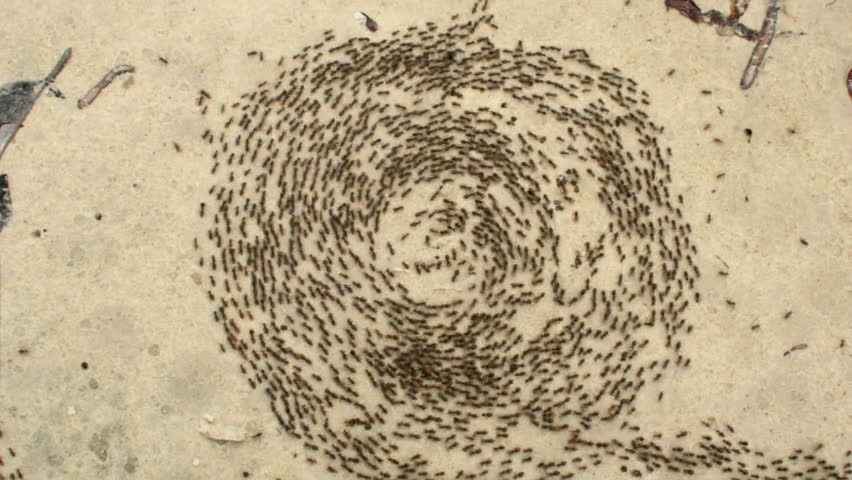
\includegraphics[width=.5\textwidth]{image/deathcircle}
\captionof{figure}{Blind army ants rely on the scent of other ants to navigate.  But sometimes they get stuck following each other into a circle without knowing that they are lost.  They eventally die as they diligently march on to what they think is the correct path.}

\background{
Warrior ants are blind and rely on the scent of other ants to navigate.  Sometimes they end up in what is called the death circle (get source or picture).  

Death Circle is like the apostasy.  A blind prophet cannot lead another blind man and both shall march in circles without hope until they die.
}

\end{entry}

\begin{entry}
\heading{Wear on Self-Worth}
\source{Tire Wear}
\background{Self actualization vs overinflated ego  and underinflated self worth}
\end{entry}



%% Book of Mormon %%
% Book of Mormon.tex
\newpage

\part{Book of Mormon}

% Helaman.tex
\section{Helaman}
\begin{entry}
\heading{Democracy}
\source{Helaman Ch 1}
\background{Pahoran the Older dies and leaves his three sons (Pahoran, Paanchi, and Pacumeni) to dispute over who becomes the new chief judge over the Nephites.}

\quote{4 Now these are not all the sons of Pahoran (for he had many), but these are they who did contend for the judgment-seat; therefore, \underline{they did cause three divisions among the people.}}

\date{4/5/16}
\thought{It is amazing how just three individiuals were the cause of such division.  We see this kind of division in politics all the time.  Two parties with one or two popular candidates each.  My perspective on this is that different oppinions are important.  We come to better conclusions when we debate ideas.  Even the 12 apostles of the Lord do not always agree on things, but they always are unified.  I think that is the difference between division and contrasting oppinions.}
\question{Can there exist healty division in a political standpoint?}
\keyword{Division}
\keyword{Politics}

\BrText{Pahoran was nominated by democracy.}{
5 Nevertheless, it came to pass that {Pahoran was appointed by the voice of the people} to be chief judge and a governor over the people of Nephi.
}
\BrText{Paanchi accepted that he was losing and joined up with Pahoran and not his other brother Pacumeni.}{
 6 And it came to pass that \textbf{Pacumeni, when he saw that he could not obtain the judgment-seat, he did unite} with the voice of the people.}
 \BrText{Pacumeni does not accept the choice of the people and stirs up trouble.}{
 7 But behold, \textbf{Paanchi, and that part of the people that were desirous that he should be their governor, was exceedingly wroth}; therefore, he was about to flatter away those people to \textbf{rise up in rebellion} against their brethren.}

\end{entry}

%% Chapter Seven %%%%%%%%%%%%%%%%%%%%%%%%%%%%%%%%%%%

%% Chapter Eight %%%%%%%%%%%%%%%%%%%%%%%%%%%%%%%%%%%
\subsection{CH 7-8 Nephi's Prayer of Lamantation}

Nephi comes back from proselyting to the lamanites to find that the Nephites have become wicked and have united with the gadiantan robbers.  He is spotted praying by the people and he confronts them about their iniquities.

\begin{entry}
\heading{Remember Him}
\source{Helaman 7:20}
\quote{20 O, how could you have forgotten your God in the very day that he has delivered you?}
\thought{It is easy to boast in our own success and forget that without the Lord's help we could not have accomplished all that we had.  For example, praying for the Lord's help to succeed in an exam and then forgetting to give thanks for aiding in remembering the material.}
\keyword{Remember}
\keyword{Forget}

\end{entry}


\begin{entry}
\heading{False Security}
\source{Helaman 8:6}

\BrText{Satan's lie of False Security.}{6 And now we know that this is impossible, for behold, we are powerful, and our cities great, therefore our enemies can have no power over us.}

\thought{Believing that you can handle temptation can similarly be destructive.  For instance, the insentive to go to a party outweighing the temptation of alcohol found there in. The same can be said about allowing pornography into your mind and expect to not be effected. }
\keyword{False Security}
\keyword{Pride}

\end{entry}
%% Old Testament %%
% OT.tex
\newpage

\part{The Old Testament}

%%%%%%%%%%%%%%%%%%%%%%%%%%%%%%%%%%%%%%%%%%%%%%%%%%%%%%%%%%%%%%%%%%%%%
\section{Proverbs}

\begin{entry}
\heading{Attitude of the Scorner}
\source{Proverbs 9:8-9}
\date{March 29, 2016}
\quote{8 Reprove not a scorner, lest he hate thee: rebuke a wise man, and he will love thee.\\
 9 Give instruction to a wise man, and he will be yet wiser: teach a just man, and he will increase in learning.}
 \thought{This scripture is about you. The attitude which you choose to bear will strongly determine your progress in life.  Will you dismiss your critic with scorn like the dog that bites the hand that feeds it?  Or do you acknowledge the wisdom in others, and love them for their faults?}
\keyword{Attitude}
\keyword{Wisdom}
\keyword{Scorner}
\keyword{Ethics}
\keyword{Learner}
\end{entry}


%% New Testament %%
% NT.tex
\newpage

\part{New Testament}

% Matthew.tex

\section{Matthew}

%%%%%%%%%% CH 7 %%%%%%%%%%%%%%%%%%%%%%%%%%%%%%%%%%%%%%%%%%%%%%%%
\begin{entry}
\heading{Faith is More than Calling on God at the Last Day}
\source{Matthew 7:21-23}
\date{April 25, 2016}
\background{Jesus' Sermon on the Mount}
\BrText{It is a weak argument to say that we spent our life on the Lord's errand when we do not seek the truth first.  There is only one God and one true church.}{21 Not every one that saith unto me, Lord, Lord, shall enter into the kingdom of heaven; but he that doeth the will of my Father which is in heaven.
~\\
 22 Many will say to me in that day, Lord, Lord, have we not prophesied in thy name? and in thy name have cast out devils? and in thy name done many wonderful works?
~\\
 23 And then will I profess unto them, \textbf{I never knew you:} depart from me, ye that work iniquity.
 }

 \thought{
 God is Just and Merciful but doesn't yield to sin.  God has given us ample time to repent of our wrong doings.  If our heart is pure, we will be given discernment as to which church is His.  The easier path is a deadend.
 
 We work iniquity when we use the Lord's name in vain and profess to act in His behalf.  In otherwords, we need to righteously hold the priesthood and use it to serve others.  Otherwise, our example can be like that of false prophets.  Let our conduct separates us from the world.
 }
 \keyword{Church, True}
 \keyword{Work}
 \keyword{Vain}
 \keyword{Last Day}
 \keyword{False Prophets}
 \keyword{Priesthood}
 \keyword{Death Bed}
\end{entry}


%% Mission Brazil %%
% Mission_Brazil_Londrina.tex
% Content:
%	Experiences, Lessons learned, Things learned by Companions
\newpage

\part{Mission Brazil, Londrina 2011-2013}
\section{Companions}
This record contains the councel I received in meetings and from other missionaries. The most important things that I learned on my mission were from the examples of my mission compainions.  This record was intended for my self-improvement as I prepare myself to become a better leader.  My intention for this book is to develop the qualities that I think are important in other people.  

Most of these entries were written the transfer after.  

\begin{entry}
\heading{Life Long Learner}
\source{E. Skillings}
\date{1st Transfer, Foz do Igua\c{c}u}
\myfigure{L}{\linewidth}{\linewidth}{image/ESkillings}{photo}{Heading back to the city after lunch with the Bishop's family on his little farm.}
\background{
Elder Skillings was my trainer.  I only had him for a companion for one tranfer, but I learned a lot from him.

The greatest things I learned from my trainer were
\begin{enumerate}
\item My time on the mission is precious.  Use it all.  Take notes, keep a revelation book, value my journal, and take advantage fo the spirit.  This is a unique experience were I can have revelations and learn things spiritually at an easier way.
\item Aspire to become something better.  To become something and stop is not the life of a missionary.  Because of this counsel, I strive to become the best missionary, and someday a great trainer myself.  I will strive for an excellence I never have before.
\item How to study effectively.  This simple teaching is to abide by the rule of focus.  Memorize, practice, constantly refresh the principle throughout the day.  This is how I learned to teach lessons in Portuguese.
\end{enumerate}

These lessons are the road to success as a missionary.  After the mission, I plan to use them in school and my continuation of learning the gospel everyday.  The mission really is the basis for the rest of my life.  It isn't a step but a foundation.  I'm grateful for my trainer Elder Skillings.  He truly is inspired and was inspired to be my trainer.  He's the man and I hope to meet up with him after the mission. 

The First Rule to the Mission:\\
Elder Skillings also taught me the first rule to the mission. "Never let the language frustrate you."  I took that to thought.  The times I got frustrated I think I was only thinkgin about myself.  I'm new.  The key is that it doesn't matter how much people understand me, just that I'm learning.  I'm not gonna speak perfectly yet.  I've only had two months in the field.

Instead, Elder Skillings taught me how to learn: memorizing passages, memorizing new words each day, read the scriptures out loud, and try to gain inspiration through the lessons.  This is my time to grow in Portuguese and in spirit and in character.  Then Practice.  We would practice in the house during compainionship study, at lunch appointments, on the street, in lessons that day and everywhere.  Practice. Practice. Practice.

Well, I discovered that this method actually works.  Memorizing lessons isn't the thing that the MTC wanted us to learn. But I found that after memorizing, practicing, and then making new phrases to practice, I can pick and choose my lesson's content.  
}
\memory{4/3/2016}{
I remember Elder Skillings for his diligent conduct as a missionary.  I viewed him as a great leader who knew how to follow with exactness.  He was a continuing learner and humble enough to keep studying Portuguese even though he was on his last two transfers.  I remember struggling to keep up with him on the cobblestone streets of Foz do Igua\c{c}u.  He never wasted time.  He was on an errand.  His example instilled in me the importance of the mission.  It wasn't my time.  It was the Lord's which had been intrusted in me.  I strived to follow his example throughout my mission.    
}
\keyword{Diligence}
\keyword{Practice}
\keyword{Learner}
\keyword{Aspire}
\keyword{Study}
\keyword{Frustration}
\keyword{Lord's Errand}
\keyword{Obedience}
\keyword{Leader}
\keyword{Trainer}
\end{entry} 

\begin{entry}
\heading{Rough Transfer}
\source{Elder Bosse}
\date{2nd Transfer, Arapongas, Paran\'a}
\myfigure{L}{\linewidth}{\linewidth}{image/EBosse}{photo}{Elder Bosse and me during one of our long walks to the outskirts of our mission area.}
\background{Elder Bosse was a Gaucho, meaning that he was from Rio Grande do Sul.  He became a senior companion with me.  I look back to my time with Elder Bosse and have to chuckle.  It certainly was an experience.  But , I learned so much from my time as his companion.  I think I grew the most from that transfer.  Some things that I want to incorporate in my character for the future when I'm a senior companion are
\begin{enumerate}
\item Assertive Leadership
	\begin{itemize}
	\item Hesitation can sometimes be confused with spiritual revelation.  Sometimes it is necessary to just make a choice.
	\item Good planning goes a long way.  Always have a backup plan.
	\item Always assess your efficiency, professionalism, and reality.
	\end{itemize}
\item Train by example
	\begin{itemize}
	\item Don't be hypocritical.  Always apply what you teach.
	\item Apply scriptures each day.  They teach with spiritual power.
	\item Be attentive about what you teach your companion.  If you end up repeating his part of the lesson, he knows that you aren't taking the lesson seriously.
	\item Regardless of status quo, companions are equal.  
	\end{itemize}
\item Time management
	\begin{itemize}
	\item Teach simply and have focus.
	\item Be organized.  Know how the lesson should progress.
	\item Adapt to needs but know priorities.
	\item Know when to move on.
	\end{itemize}
\item Caring for the People
	\begin{itemize}
	\item Practice lessons well.
	\item Know how to follow-up with addictions.
	\item Know priesthood ordinances well.
	\item When you find a doubt in a person (or create it), seek to solve it.
	\end{itemize}
\end{enumerate}
I think the most important lesson I learned was that we are growing up on the mission.  However, your shoes are paving a path.  We are pioneers for other missionaries.  We need to treat our companions as filling our shoes one day.  Prem them to carry out the work through example and concern yourself with their success.
}
\memory{April 3, 2016}
{I was unfair to Elder Bosse. During my time with him, I felt like he was limiting me.  When he moved out, three new missionaries lived in my home and I told them all of the negative things that Elder Bosse had done during his transfer with me.  Finally, Elder Morell said after weeks of hearing me, "Man, you say such negative things about your companion.  I'd hate to imagine what you'll say about me." I felt sick of what I had done.  How the power of ill-speaking had gripped me to destroy the image of a fellow missionary.  Another individual that had given up two years of his life to serve the Lord to the best of his ability.  I never spoke ill about him or any other companion since.  What a great lesson I had learned.  Now that I am married, it continues to be enforced. }
\keyword{Gossip}
\keyword{Example}
\keyword{Assertive}
\keyword{Time Management}
\keyword{Charity}
\end{entry}

\begin{entry}
\heading{Influencial Speaker}
\source{Elder Da Rita}
\date{3rd Transfer, Arapongas, Paran\'a}
\myfigure{L}{\linewidth}{\linewidth}{image/EDaRita}{photo}{Elder Da Rita and me standing in front of the chapel the day before transfers right after learning that he would be training a new missionary and I would be transferred to Presidente Prudente.}
\background{
Elder Da Rita was a short carioca missionary from Rio.  He was a very influencial missionary and gave great speaches.  I'm grateful for the opportunity of serving with Elder Da Rita.  He was very inspirational and showed me how to become a more active missionary.  the things I learned from my experiences with him are priceless in my daily life as a missionary.  I learned and watched how he taught people.  He could break people down and pull out the raw material that made them the way they are.  He had the ability of reading people like a book.  I learned that you need to start with the basic questions.  How did things happen?  How did you meet the missionaries the first time?  Why did you initially join the church?  How long have you stopped going?  He took the time to understand their condition before prying at them and trying to get them to go to church.

I also found that you need to get to know the members.  The members are the key to helping investigators.  You must know how to use them.  

Don't judge people until after you teach.  A lot of cool people tend to look dull and the adversary wants hinder us by making us think that they will waste our time.  Bust Jesus wasn't sterotypical.  Everyone has problems.  We are here to ease the burden of others.  Why not help people that are without the gospel?  

Be united with your companion.  Your communication needs to be united.  Teach united.  Feel unity.  Need unity and balance in your relationship with your companion, roommates, members, and everyone else.  That's the road to success.  

He really knew how to raise people's spirits.  Especially those with addictions.  "Never give up!"  "We need to keep trying because our salvation is on the line!"  Elder Da Rita was encouragement.  I'll keep in practice the things I learned from him throughout the mission.  Just have a good attitude and get to work.}
\keyword{Influence}
\keyword{Inspire}
\keyword{United}
\keyword{Attitude}
\memory{April 3, 2016}
{A phrase that Elder Da Rita always said was "Nunca desistir" and also "Depende de cada um de n\'os."  Translated meaning, "Never give up" and "It depends on every single one of us."  Instilling hope in those that need it was one of those traits that Elder Da Rita had. Once we met with a senior woman that had a leg amputated.  She was in great distress.  We came in and visited for a while and then offered to give her a blessing so that she wouldn't lose her other leg.  The next time we visited, both legs were gone.  There was a strong emotion in the atmosphere as she wept about her loss.  Yet, Elder Da Rita told her to be peaceful and never give up.  We offered a prayer in her behalf.  That experience was very impactful in my life.}
\keyword{Hope}
\keyword{Priesthood}
\memory{April 3, 2016}
{The senior woman had a friend who lived nearby who was there during our visit.  She was impressed by us and invited us over.  We marked an appointment and left it as that.  The day came and we had spent the whole day being turned away.  Every appointment fell.  The day before our lead investigator told us that she was moving but we found her hiding from us as we passed by that day.  Elder Da Rita got really down about it and we ended up forgetting our appointment with the lady.  We went back the next day to appologize and see if we could still visit her.  She then asked, "Where were you guys?"  We gave her our response to which she said, "I invited all of my friends over to hear you guys.  I had almost thirty people here waiting for you but you never showed up."  Undoubtably, we both felt really bad.  We could have had thirty new investigators in a single lesson!  I remember Elder Da Rita commenting to me that he admired my attitude to never get dissappointed.  Even on the downest days I could shrug it off.  As the years pass, I realize how crucial that characteristic is.  We cannot get down about our situations because we may miss a very special blessing prepared for us.} 
\keyword{Dissappointment}
\end{entry}

\begin{entry}
\heading{The Patient Teacher}
\source{Elder Teixeira}
\date{4th Transfer, Presidente Prudente, S\~ao Paulo}
\myfigure{L}{\linewidth}{\linewidth}{image/ETeixeira}{photo}{Elder Teixeira and me standing on the top of our apartment complex overlooking the city of Presidente Prudente.}
\background{
Elder Teixeira was someone that built me up a lot.  I grew a lot the transfer with him.  I loved him so much and wanted to become the best missionary possible.  We had lots of fun while being focused on the mission.  He really was an awesome missionary.

The things that I learned from Elder Teixeira will always be a blessing for me in my life.  I learned
\begin{enumerate}
\item How to teach all the lessons really direct and simple.  And care for them.  He showed how to act toward our investigators to get them to open up.  You have to get to know them, show them that you care for them and their family, and always pass by.
\item Patience.  He taught me this when I got frustrated at the other missionaries for making us waste a few minutes of P-day waiting for them.  I learned that a little bit of patience goes a long way in a relationship.  You build unity through patience.
\item He taught me to be a senior.  He had me guide days and experiment being in charge.  I learned a lot of qualities of being a leader during my transfer with Elder Teixeira.  Because he was such a great one.  
\end{enumerate}
I hope to one day be as good a missionary as Elder Teixeira.  He was just on the ball with everything.
}
\memory{April 3, 2016}
{One thing that I remember about Elder Teixeira was his eagerness to teach.  He was always smiling and finding a reason to laugh.  Not only did he want to teach well, but he was organized at it.  He was a bit OCD.  But when he realized that I was serious about learning Portuguese, he got excited and helped me learn words and practice lessons effectively in the language.  We would practice on the road teaching lessons to each other.  I finally felt like I was getting a grasp on the language when he was my companion.  He even helped me with my accent.  

Another important memory item was that he would focus on getting me to become a leader.  He knew that he was leaving the area soon and that I would likely stay and would need to know the streets and how to organize a day for my new companion.  His planning style has continued with me even to college.  I feel like planning is a key in success.

His patience also astounished me.  I'm a very impatient person.  But I learned how to be more patient because of him.  He was a great example of waiting on others even though he had plans already made.  When the missionaries took up part of my P-Day (maybe five minutes) he told me to just be a little more patient.  I wasn't and went and told them that I was upset with them.  Back in the appartment, he told me that the missionary that I had said that to looked up to me and thought highly of me.  I naturally felt bad about it and ended up trying to make it up to him and we became great friends.  A little patience and understanding goes a long way.}
\keyword{Patience}
\keyword{Teacher}
\keyword{Plan}
\keyword{Organize}
\keyword{Unity}
\end{entry}

%%%%%%%%%%%%%%%%%%%%%%%%%%%%%%%%%%%%%%
%% ELDER DOUGLAS
%%%%%%%%%%%%%%%%%%%%%%%%%%%%%%%%%%%%%%
\begin{entry}
\heading{Three Transfers of Glory}
\source{Elder Douglas}
\date{5-7th Transfers, Presidente Prudente, S\~ao Paulo}
\myfigure{L}{\linewidth}{\linewidth}{image/EDouglas}{photo}{A regular day with Elder Douglas.}
\background{
Hmm... where to start.

Elder Douglas was my companion during some of the most challenging times of my mission and he helped shape me to be who I am now.  he once told me that he doesn't take friendships lightly; a friend is part of him.  I feel the same way.  Elder Douglas is now a part of who I am.

Four and a half months is a long time to be stuck with the same person day in and day out.  I really got to know him well.  One thing that I admired about Elder Douglas was his abiliy to share stories.  He could relate anything to the gospel.

When we started off, we were working our tails off for baptisms.  We worked super hard.  But the thing that caught my attention was the expression of faith he had.  He would truly walk (if not run) by shear faith.  

Treating people how you want them to be, not how they are.  He took that to heart and we both learned a big lesson about that as we worked with the branch leadership.

Importance of a name.  Leadership skills were a priority to him.  He always wanted to get to know people before hearing numbers.  He taught me that learning people's names is really important to them.  It is respect.

Put the goals in your heart.  Think them, breath them, just get them done.  Diligence at its max.

Elder Douglas was also the most genuine missionary I met.  Super sincere.  Here for the right cause.

Rules equal power.  He never justified the rules.  He wanted and needed the spirit.

Life isn't easy nor hard; it's fun.  We all pass through tough times.  They pass.  And we become stronger.

Use experiences and talents of others for good.  Note their abilities.  Ask for guidance.  Don't try to just go about it by yourself.}
\keyword{Big Harry Audacious Goals}
\keyword{Just Do It}
\keyword{Unity}
\keyword{Prayer}
\keyword{Friend}
\keyword{Faith and Works}
\keyword{Goals}

\memory{xxx}{
Praying for mountains to climb.}

\end{entry}

\begin{entry}
\heading{My Chilean Friend}
\source{Elder Quijada}
\date{8th Transfer, Mar\'ilia, S\~ao Paulo}
\background{
My chilean companion of power!

I became senior companion the transfer with Elder Quijada, wo it was kind of a test run as leader for me.  He reminded me a lot of myself six months earlier.  He's a great missionary that wants to do good.  Wants success.  And is diligent.

I realized that attitude and respect are closely linked to each other.  And I began to get a taste of my own medicine with Elder Quijada.  With Elder Douglas I felt like I knew better than him.  With Elder Quijada, it felt like I was dealing with myself.

Good plans let God prepare a way for you to find elects.  Need to be flexible as a person though.  Because of our plans we ended up in the right place at the right time even though things fell through.  We found a nice family and they ended up getting baptized.

Careful with gestures.  They provoke bad attitudes and display a lack of respect.  Be careful when you get aggitated or frustrated.

I learned most of all to be chill.  Turst in God.  Help your companion build faith by diligence and prayer and acknowledging God's hand in your success.}
\keyword{Planning}
\keyword{Spirit, Guided By The}
\keyword{Karma}
\memory{April 23, 2016}{
Elder Quijada and I were tracting and came to a door.  As we talked to the guy that lived there, it was apparent that he was not interested in our message and started to debate/question our doctrine.  My companion lost his temper and began to "bible-bash" with the man.  I wanted to control the situation so I took over and had to apologize to the man for my companion's remarks.  The guy was offended and rejected my offer to visit the church to learn more.  

While I had been trying to fix the situation, Elder Quijada had wandered down the street a few houses.  When I caught up he went off on how I was wasting the Lord's time with that man.  In English, I made a mistake and told him to "shut-up" out of frustration.  He recognized the term and blew up on me. In the heat of the moment, I told him that we were going to initiate an inventory that very moment in the street.  Fortunately, there weren't many people passing through the street to over hear our conversation.  I asked him to pray.  I started the meeting by telling him that he was an outstanding missionary and that I appreciated his diligence and great ability to teach the gospel.  He really was well versed in the doctrine.  But I told him that he lacked respect.  I felt that he, like I had in previous transfers, felt entitled to lead and disregard his companion's opinion.  I told him that it didn't work that way.  We both needed to work together.  I also apologized for my language and told him that I respected him.  

I had him talk about his thoughts about me as his companion.  He told me that he really did like me as a companion and that I was driven to meet my goals which his previous companions had fallen short of.  He gave me some advice too.  In the end, we both felt firm in our relationship and we were able to continue tracting.  

It was a great transfer together and we both learned a lot together.  
}
\keyword{Bible-Bash}
\keyword{Inventory}
\keyword{Respect}
\keyword{Unity}
\keyword{Attitude}
\end{entry}

\begin{entry}
\heading{The Light}
\source{Elder Gutemburg}
\date{9th Transfer, Quebec, Londrina, Paran\'a}
\background{
Man I learned a lot with Elder Gutemburg. He is a mineiro meaning that he is from Minas Gerais. During my time with him, I learned the importance of being an example.  If I want respect, I have to give it first.  Also, he's a convert of about two years.  My focus was to build up his faith.

Something that I figured out, as I tried to help him become better, was that all of my tips and critiques came out wrong.  I learned that you need to be a light not a judge.  I tried to tell him what he needed to change, but it was the things he saw me do that really made the difference: how I worked, treated others, studed, etc., where the things he began to incorporate into his life.

Be a light.}
\keyword{Light}
\keyword{Example}

\memory{April 23, 2016}{
I remember Elder Gutemburg talking about how he held missionaries at the highest esteem as a convert.  But when he entered the mission field, he realized that they were less than perfect.  I've thought about his experience a lot and how it had troubled him.  I think missionaries have that kind of impact on the people that they come in contact with.  It is depressing to think that the hard work of many missionaries can be dismissed by the ill-set example of a few individuals that have not yet mutured and fool the world around them that they are heaven sent.  Missionaries are not sent by God to raise up injust acts of self-centered adolescents.  Though a mission can change a person from good to better, it can often make a person bad turn to the worst.  Preparation is key.  Missionaries need to be better equipped with the gospel.  That means that they not only know the gospel, but they have a living testimony of it, aka they live it.  They stand by it.  They live and breath by the power of obedience.  They keep the Savior's name written in their hearts by sustaining their church leaders and holding fast to their covenants.  

Gossip is also not besseting of missionaries.  Elder Gutemburg told me mid-transfer that I was nothing like he had been told.  His previous companion, who I had met once prior, had convinced him that I was a lazy missionary and very dumb and that he would have a rough transfer with me.  Elder Gutemburg said to me that he had been deceived and that he believed now that his previous companion fit that discription better, now that he had the facts.  In fact, he told me, because of how diligent I was regardless of the situation I was in, he felt immensly better about being a missionary.  The sick feeling of throwing away his mission the transfer before by doing nothing all day had dragged on his mind.  As he became more diligent he felt the spirit everyday the transfer he was with me.  It made me grateful to know that I had made that change in his mission.  His next transfer he was able to baptize more than a dozen individuals.  I believe that the spirit of missionary work had inspired him to be better and he was inclined to be the best he could.  
}
\keyword{Gossip}
\keyword{Missionary Standards}
\keyword{Righteous Judgment}
\keyword{Self-Fulfillment}
\end{entry}

\begin{entry}
\heading{Support from my Side}
\source{Elder Saraiva}
\date{10-11th Transfers, Quebec, Londrina, Paran\'a}
\background{
I think the greatest trait that Elder Saraiva had was submissiveness.  I never saw him, for the two transfers together, ever get mad.  He was willing to work, plan, and aim for good goals.  

What I learned from Elder Saraiva:
\begin{itemize}
\item Unconditional love.  We did things for one another.  He would make food for me.  We just had a great friendship.
\item Repetition.  He would always repeat things.  It drove me crazy at first, but then I realized it is the best way to learn and remember.
\item Cultural differences.  man, we had a lot.  At times it got in the way.  but we learned to break the barriers.
\end{itemize}

I love Elder Saraiva.  My junior companion that never whined!  He was such a great support.  I felt like I needed support from above in order to finish my mission out strong.  But I realized that what I really needed was a supporting companion that helped lead and strove to be his best.
}
\keyword{Repetition}
\keyword{Support}
\keyword{Love}
\keyword{Attitude}

\end{entry}

\begin{entry}
\heading{Baptism by Fire}
\source{Elder Pereira}
\date{12th Transfer, Camb\'e, Paran\'a}
\background{
I only stuck with Elder Pereira for two weeks due since I needed to be relocated to the mission home for medical reasons, but I learned a lot.  Of all the things about him, I loved teaching with him.

The most important and humbling thing that I learned with Elder Pereira was that I should never judge someone without any prior knowledge.  I did not have all of the puzzle pieces to understand how a person is how he is.  

I also learned how to forgive and ask for forgiveness faster; to not escalate bad feelings or let them grow untended like weeds in a garden.  I think this is also a quality that my dad has perfected: patience and forgiveness through long suffering. 
}
\memory{xxx}{My bad attitude and his family life.  The silent treatment}

\memory{xxx}{Getting sick and travelling to the hospital.}
\end{entry}

\begin{entry}
\heading{Sick at Work}
\source{The Secretaries}
\date{12th Transfer, Ala 1, Londrina, Paran\'a}
\background{
After getting sick, I spent the rest of the transfer in Londrina with the secretaris.  I learned a lot from each one:

Elder Childs:\\
He was always searching the scriptures and making connections with gospel topics.  It was really fun to learn about his insights of the gospel.  He had a stamp with the word "Docrine" on it that he would use to stamp things that he really liked in his scriptures.  He was also mindful of peoples needs and had a joy in learning.

Elder Furtado:\\
He always got to know people and their interests.  He liked to share things and was hard to get offended by others.  He would go the extra mile and sacrifice personal time for others.

Elder Watson:\\
He had a great desire to become like the other missionaries that he lived with and wanted to learn more about the gospel.  His desire to learn and follow were important.

Elder De Araujo:\\
He was very prayerful.  He would pray daily for many minutes during scripture study.  He sought self-perfection which allowed him to learn from others when they gave him feedback.  One important thing that I liked from him was the attitude of finding out if something is right or wrong before acting rather than the attitude of doing it until told otherwise.
}

\end{entry}

\begin{entry}
\heading{Funny Argentino}
\source{Elder Guebara}
\date{13th Transfer, Centro C\'ivico, Londrina, Paran\'a}
\background{
Elder Guebara helped me a lot.  Aside from being my funniest companion on the mission, he helped me see that I needed a better attitude.  He would always say things like "not with that attitude it won't happen."  My attitude was dragging me down.  I needed to do two things:
\begin{enumerate}
\item Stop being angry with the leaders and questioning whether they were really called of God.
\item Be ok with my position in the mission.  I may never be a "leader" in the mission, but think about the blessing it is just to be a missionary.
\end{enumerate}
I needed him as my companion.  He really helped me understand my role and purpose as a missionary.
}
\keyword{Attitude}
\keyword{Called}
\keyword{Blessing}
\keyword{Worry}
\end{entry}

\begin{entry}
\heading{Last Transfer in Londrina}
\source{Elder Doan}
\date{14th Transfer, Centro C\'ivico, Londrina, Paran\'a}
\background{
I loved Elder Doan.  He was awesome.  He always ironed my shirt for me, or shined my shoes, or made me food.  He was a great companion.

I realized that through my example, I could talk about my experiences in a way to encourage him.  For example, I always was happy and diligent.  So when I told him that I, like him, had hardly ever baptized on the mission, he realized that he could relate and feel confortable carrying on.  In fact, I taught him some of the wisdom that I had learned on my mission.  I told him, if your goal on the mission is to baptize 100 people before you're through, then you will only find success after the 100th baptism.  Even 99 baptisms would be a failure.   But if you define success inline with the Lord's definition, the outcomes are different.  If you come out more Christ-like, more diligent, patient, having charity for strangers, you will be successful.  If you do your best each day to spread the gospel and you are progressing and not going backward, you are a successful missionary.  Carry on.   

From him, I learned to be a little more responsible.  But most importantly, I learned to be a true companion that loves and respects the other.  he was truly a supurb example to me.
}
\keyword{Carry On}
\keyword{Success}
\keyword{Progress}
\keyword{Diligence}
\keyword{Long Suffering}
\end{entry}

\begin{entry}
\heading{One Last Mountain}
\source{Elder Gregory}
\date{15-16th Transfers, Bela Vista, Bauru, S\~ao Paulo}
\background{
Elder Gregory was my last companion on the mission.  I know that my time with him was worth every challenge.  My focus as his companion was comprised of two things:
\begin{enumerate}
\item Become compatable missionaries that are dedicated to the same task and, not only self-reliant, but also dependent on one another.
\begin{itemize}
\item This was hard.  We had many differences.  But I wanted it to work.  it needed to be mutual.  I learned that it is one thing to learn how to teach with another person, but another to cope with intolerance.  I found that communication was the key.  I also learned that reality is hard to communicate unless you tell your feelings and show the truth behind the situation.  For instance, giving the silent treatment is never beneficial to a relationship.  Talk about your problems and get them figured out.  Be willing to make changes as well.  This doesn't mean be passive but rather be moldable.  Recognize that you are both learning.
\end{itemize}
\item How to prepare your companion for leadership.  I realized that all of my junior companions were on the verge of becoming senior companions and even leaders.  I tried my best to put them in my shoes.  And they did well at following. 
\begin{itemize}
\item Its about the basics.  A principle of "hitting the mark."  That means knowing the purpose of all tasks, focusing on attaining that purpose, and sacrificing yourself for that cause.  For example, when we study in the morning for one hour, what is the purpose?  To prepare people to be baptized and converted to the gospel through the Spirit.  If you spend that time studying about the Lectures of Faith and "Deep Doctrine," which is not breaking any rules, are you focused on the purpose?  No.  You lose the purpose.  And with it, you lose the cause and your sacrifice is vain.  
\item I tried explaining this to Elder Gregory but he was bent on his own methods.  He didn't get it.  Oh well.  Did my part.  But I did find a way to help him see true dedication when we skipped many studies to help one individual get baptized.  
\end{itemize}
\end{enumerate}
I was bold throughout those two transfers.  I did not tolerate adolescent behavior and I did not want to waste my last precious months of the mission babysitting. 

I learned to be a better man.

Elder Gregory grew a lot.  I saw his progress.  His vision expanded.  My vision too.  We truly worked hard together.  We were both learning and growing together.  Maybe it felt like we were going backwards at times, but we were really going onward.  
}
\keyword{Bold}
\keyword{Purpose}
\keyword{Rebellious}
\keyword{Silent Treatment}
\keyword{Sacrifice}
\keyword{Mutual}
\keyword{Prepare}
\keyword{Leadership}
\keyword{Deep Doctrine}
\keyword{Role}
\end{entry}

\section{Other Experiences}

\begin{entry}
\thought{
Patriarchal Blessing

Maybe have another folder for this, but talk about how it didn't come true but then I looked at it in a different lens.  I also realized my impact on the lives of my companions rather than my flipping inactive converts.
}
\end{entry}

%\end{multicols*}

\pagenumbering{Roman}
\printindex
\end{document}